\input preamble.tex
\noindent
\section*{Læringsoppdrag Ultralydtransmitter}

\vskip 5pt
%beskrivelse av oppgaven
I dette læringsoppdraget skal du bygge en ultralyd transmitter. Først skal du koble opp og lære om hvordan de ulike delene av transmitteren virker, så skal du selv sette sammen delene til en transmitter. Du kan til en vis grad velge nivå, ved å velge hvor mange valgfrie funksjoner du legger inn i den ferdige transmitteren. 

Før du  starter med å sette sammen til en transmitter skal du utføre følgende oppkoblinger mot arduino Nano:
\begin{itemize}[noitemsep]
	\item HC-SR04 ultralyd distanse sensor. 
	\item Oled display
	\item ADC MCP4725
	\item pushbutton rotary encoder
\end{itemize}

\vskip 5pt 
Valgfrie oppdrag:

\vskip 5pt 
\begin{itemize}[noitemsep]
	\item spenning til strømkonverterer
	\item RS-485 kommunikasjon med Modbus RTU
	\item Funkjon for kalibrering til ny  tank. (Toppnivå og bunnnivå)
	\item Bytte Arudino nano med ESP32 og sette opp HMI på node-red
\end{itemize}

<++>

\vskip 2.5pt 
%kompetansemål som oppgaven dekker
Kompetansemål:
\begin{itemize}[noitemsep]

	\item planlegge, utføre, vurdere kvalitet, sluttkontrollere og dokumentere arbeidet
	\item planlegge, programmere, montere og idriftsette programmerbare styresystemer
	\item endre og tilpasse skjermbilder for grensesnitt mellom menneske og maskin
	\item anvende ulike elektroniske kommunikasjonssystemer i automatiserte anlegg
	\item vurdere datasikkerhet i automatiserte anlegg
	\item montere, konfigurere, kalibrere og idriftsettelse digitale og analoge målesystemer
	\item måle fysiske størrelser i automatiserte anlegg
	\item feilsøke og rette feil i automatiserte anlegg
	\item dokumentere egen opplæring i automatiseringssystemer
\end{itemize}

%anbefalt lesning til arbeidsoppdragene
Anbefalt lesning:

\begin{enumerate}
	\item afgv.pdf/ 
\end{enumerate}

%Liste over oppdrag som skal gjøres med ruter for godkjennening

%\begin{center}
%\begin{tabular}{ | m{10cm} | m{1cm}| m{2cm} | } 
%\hline
%\multicolumn{3}{|c|}{Liste over oppgaver som skal utføres} \\
%	\hline
%	Oppgave	& Utført & Signatur \\ 
%	\hline
%	\hline
%	(Nivå 1)	& & \\ 
%	\hline
%	(Nivå 2)	& & \\ 
%	\hline
%	(Nivå 3)	& & \\ 
%	\hline
%	(Nivå 4)	& & \\ 
%	\hline
%\end{tabular}
%\end{center}

%--------------------------------------
\newpage

\subsection*{Oppgave 1 -  Oppkobling av HC-SR04}
I denne oppgaven skal vi bli kjent med ultralydsensoren HC-SR04. Denne sensoren sender ut en ultralyd puls når Trig pinnen akriveres (10µs puls), sammtidig som trig pinnen aktiveres slås echo pinnen på, den står på til vi mottar et retur signal (reflektert lyd)

$$\includegraphics[width=9cm]{./lUltralydtransmitterx03.eps}$$
I vårt program kan vi bruke funksjonen \verb|pulseIn()|. Denne funksjonen tar tiden på hvor lenge en variabel (echo pinnen) har vært høy. Den virker på pulser fra 10µs til 3 minutter. Tiden den returnerer er i µs. 
\vskip 2.5pt 

Du kan starte med å koble sammen Arduino Nano og HC-SR04 ultralyd sensor slik:
$$\includegraphics[width=8cm]{./lUltralydtransmitterx04.eps}$$
Skriv inn denne koden i Arduino IDE og legg den inn på en Arduino Nano. Det er mulig du må bruke old bootloader. Prøv dette om opplasting ikke virker. 
$$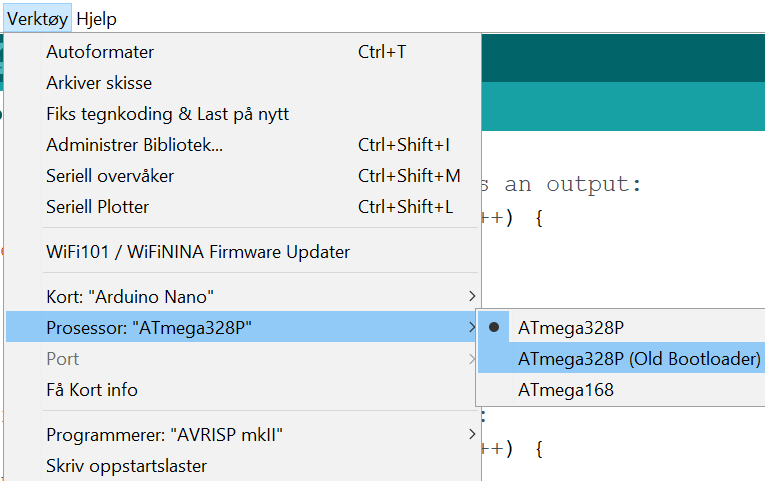
\includegraphics[width=10cm]{./lUltralydtransmitterx05.png}$$
\newpage
\begin{lstlisting}[language=Arduino]
// define the pins used for the HC-SR04.
const int trigger = 11;
const int echo = 10;

void setup()
{
	// set pin functions
	pinMode(trigger,OUTPUT);
	pinMode(echo,INPUT);
}
void loop()
{
	//first we trun off the trigger pin to be sure we have a clean high pulse
	digitalWrite(trigger, LOW);
	delayMicroseconds(2);
	//turn on the trigger pin for 10us
	digitalWrite(trigger, HIGH);
	delayMicroseconds(10);
	digitalWrite(trigger, LOW);
	// get time echo pin is on
	long duration = pulseIn(echo, HIGH);
	//recalculate time to distance
	float distance = duration * 0.0343 / 2;
}
\end{lstlisting}

Nå skal du ha et program som virker, men du har ingen måte å testet det på. Legg til funksjonalitet i programmet som gjør at du kan lese avstanden ut på seriemonitoren. Prøv også  å plotte den ut som en kurve. 

\subsection*{Oppgave 2 -  Oppkobling av 0.96" oled display}
I denne oppgaven skal vi legge til et display, dette skal brukes til å vise den målte avstanden. 


\vskip 5pt 
Displayet vi skal bruke et et 0.96" oled monochrom display. Vi kobler det til Arduino Nano ved hjelp av en buss som kalles I²C

\vskip 5pt 
-----------------Fra wikipedia------------------

\vskip 5pt 
I²C står for Inter-Integrated Circuit og er en fler-bruker seriell databuss utviklet av Philips semiconductors (i dag NXP Semiconductors) 1982, opprinnelig for bruk internt i TV-er. Nå brukes I²C for å koble lav-hastighets tilleggsenheter til f.eks. mikrokontrollere. Slik utstyr kan blant annet være display eller minne.

\vskip 5pt 
I²C er et master-slave system og bruker to bidireksjonale open-drain linjer, seriell data (SDA) og seriell klokke (SCL), som trenger pull-up motstander. Typisk arbeidsspenning for et I²C system er +3,3 V eller +5 V, men andre spenninger kan også forekomme. I²C har en 7-bits adresse, men 16 av adressene er reservert, så det er 128–16=112 noder som kan kommunisere på samme bussen.

\vskip 5pt 
I²C kan operere med flere hastigheter, de mest vanlige er standard mode, 100 kbps, low-speed mode, 10 kbps, men det finnes også fast mode plus, 1 Mbps, og high speed mode, 3,4 Mbps. De sistnevnte har også andre tilleggsfunksjoner, som bla. 10-bits adressering. I tillegg til at det maksimale antall noder er begrenset av adresser, kan ikke den totale kapasitansen på bussen overskride 400 pF.

\vskip 5pt 
-----------------Fra wikipedia------------------
\vskip 5pt

I denne oppgaven kan du koble opp slik:
$$\includegraphics[width=9cm]{./lUltralydtransmitterx0201.eps}$$
Her ser du at det vil bli litt vanskelig å koble 5V og GND til flere plasser. Da kan du ta flere koblingsledninger og lodde sammen og ta en krympestrømpe over.

\newpage
Gjør følgende:
\begin{itemize}[noitemsep]
	\item Finn frem så mange ledinger du trenger
	\item klipp av i ene enden
	\item avisoler i den enden du klipte av
	\item tvin sammen 
	\item lodd 
	\item finn passende lengde på krympestrømpen
	\item tre på
	\item krymp med varmluftspistol(lodde bolt)
\end{itemize}



$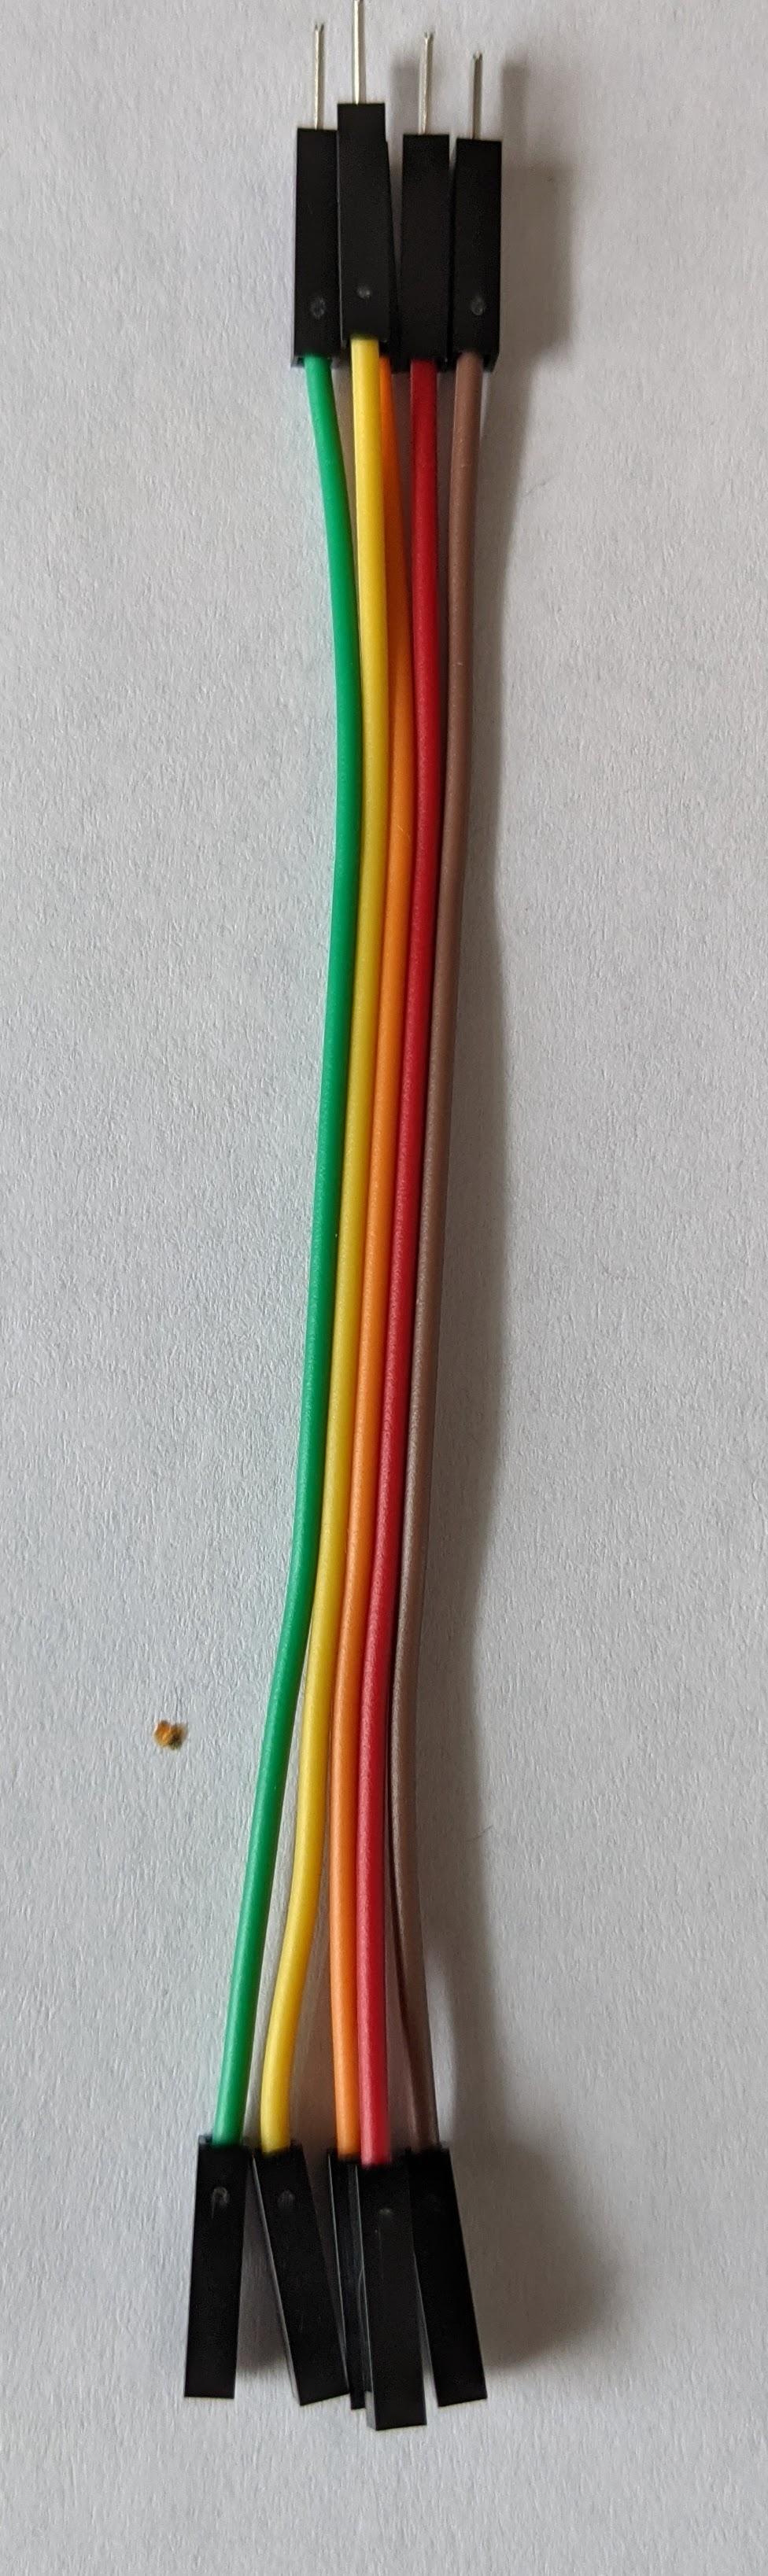
\includegraphics[height=6cm]{./lUltralydtransmitterx0211.jpg}$
$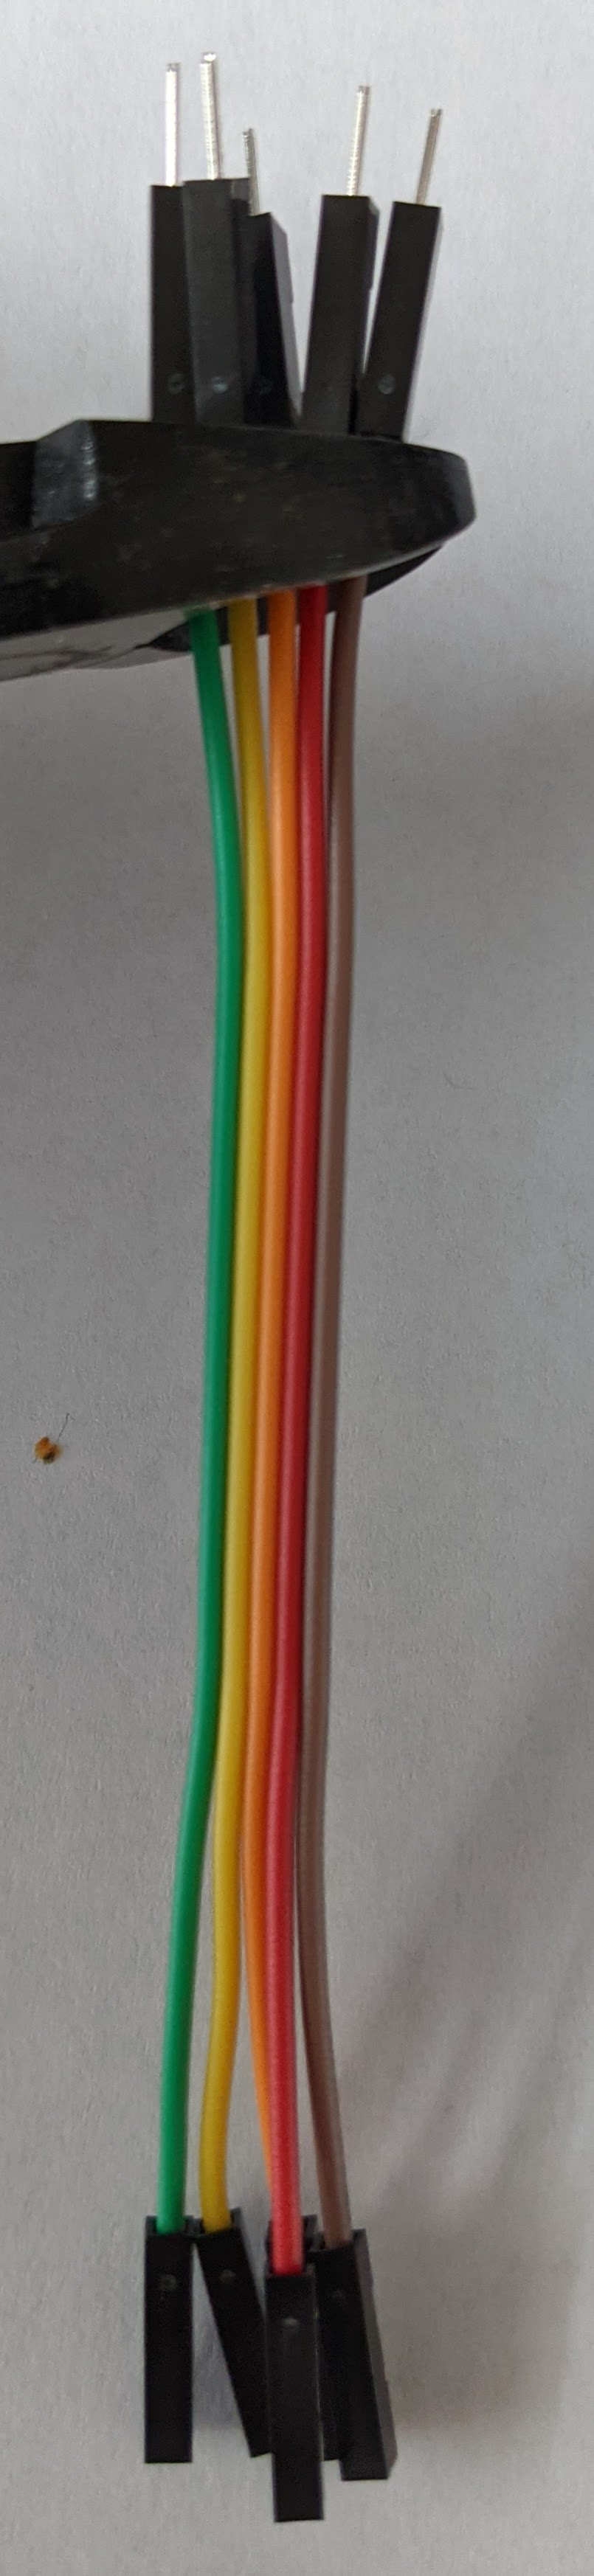
\includegraphics[height=6cm]{./lUltralydtransmitterx0212.jpg}$
$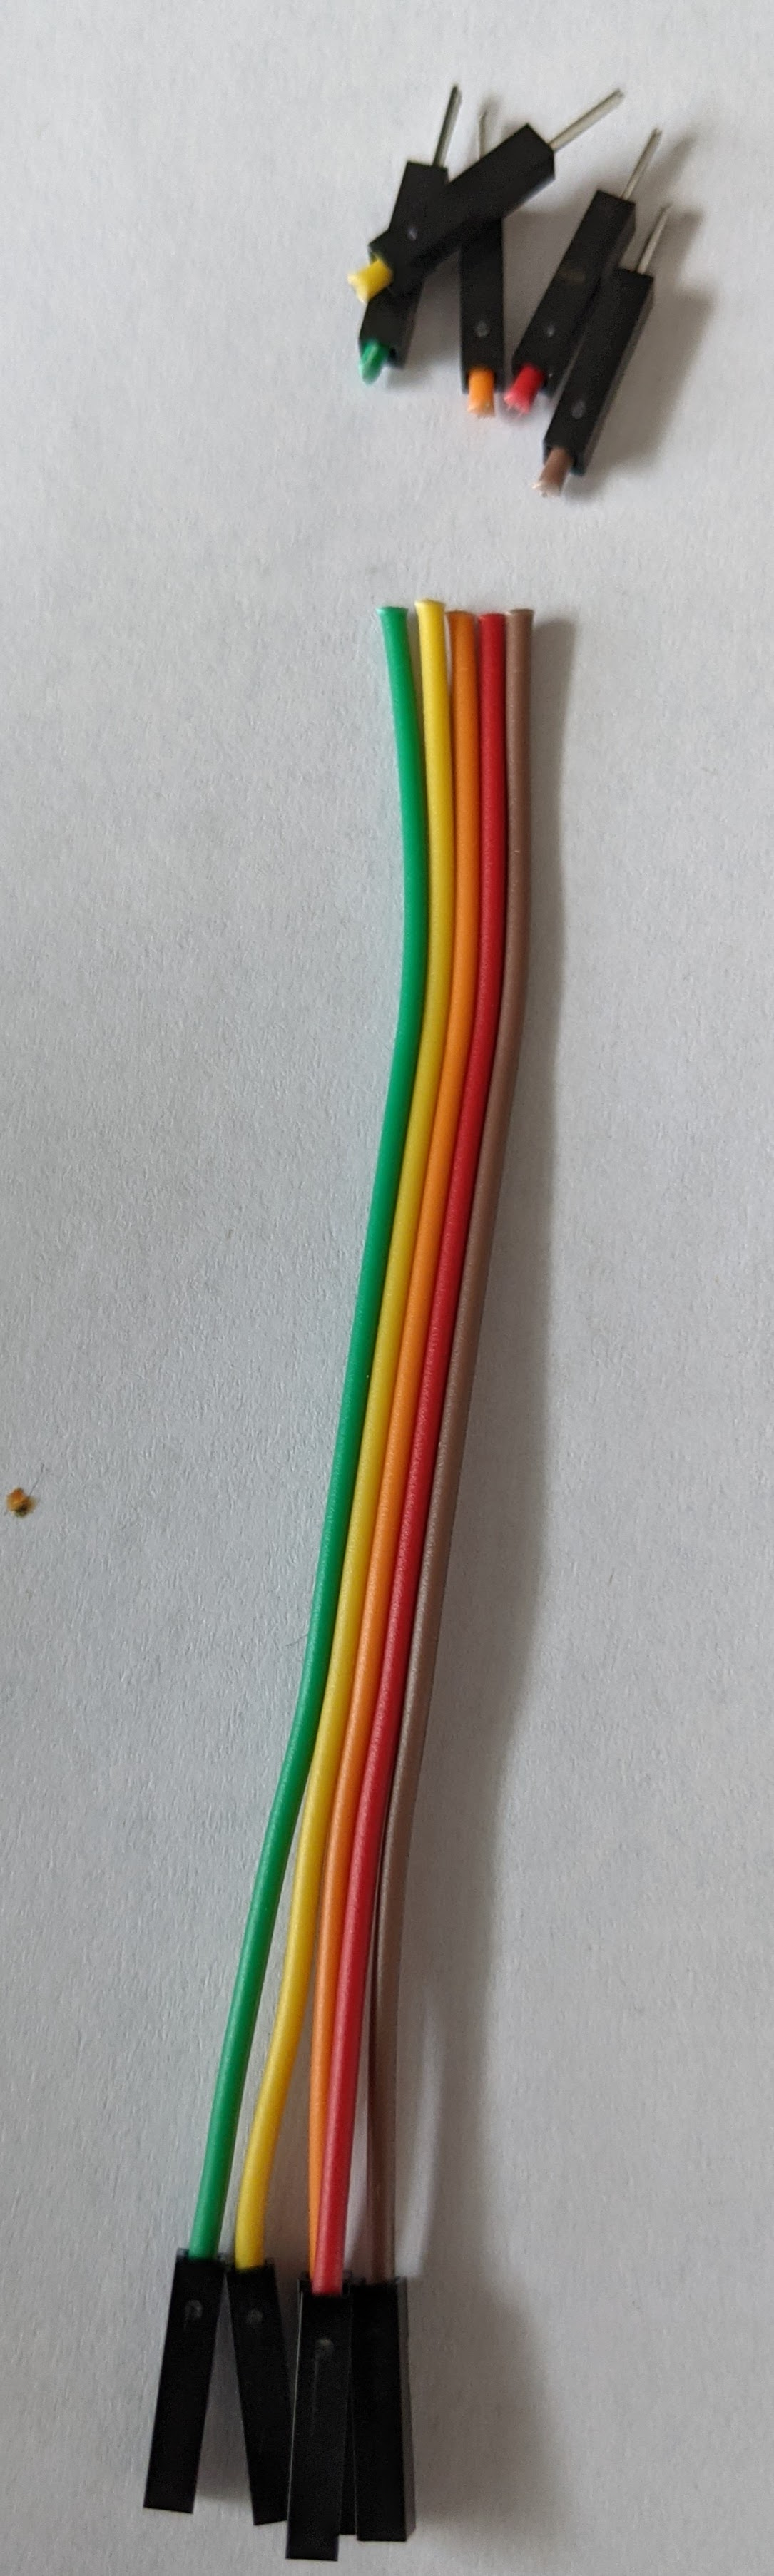
\includegraphics[height=6cm]{./lUltralydtransmitterx0213.jpg}$
$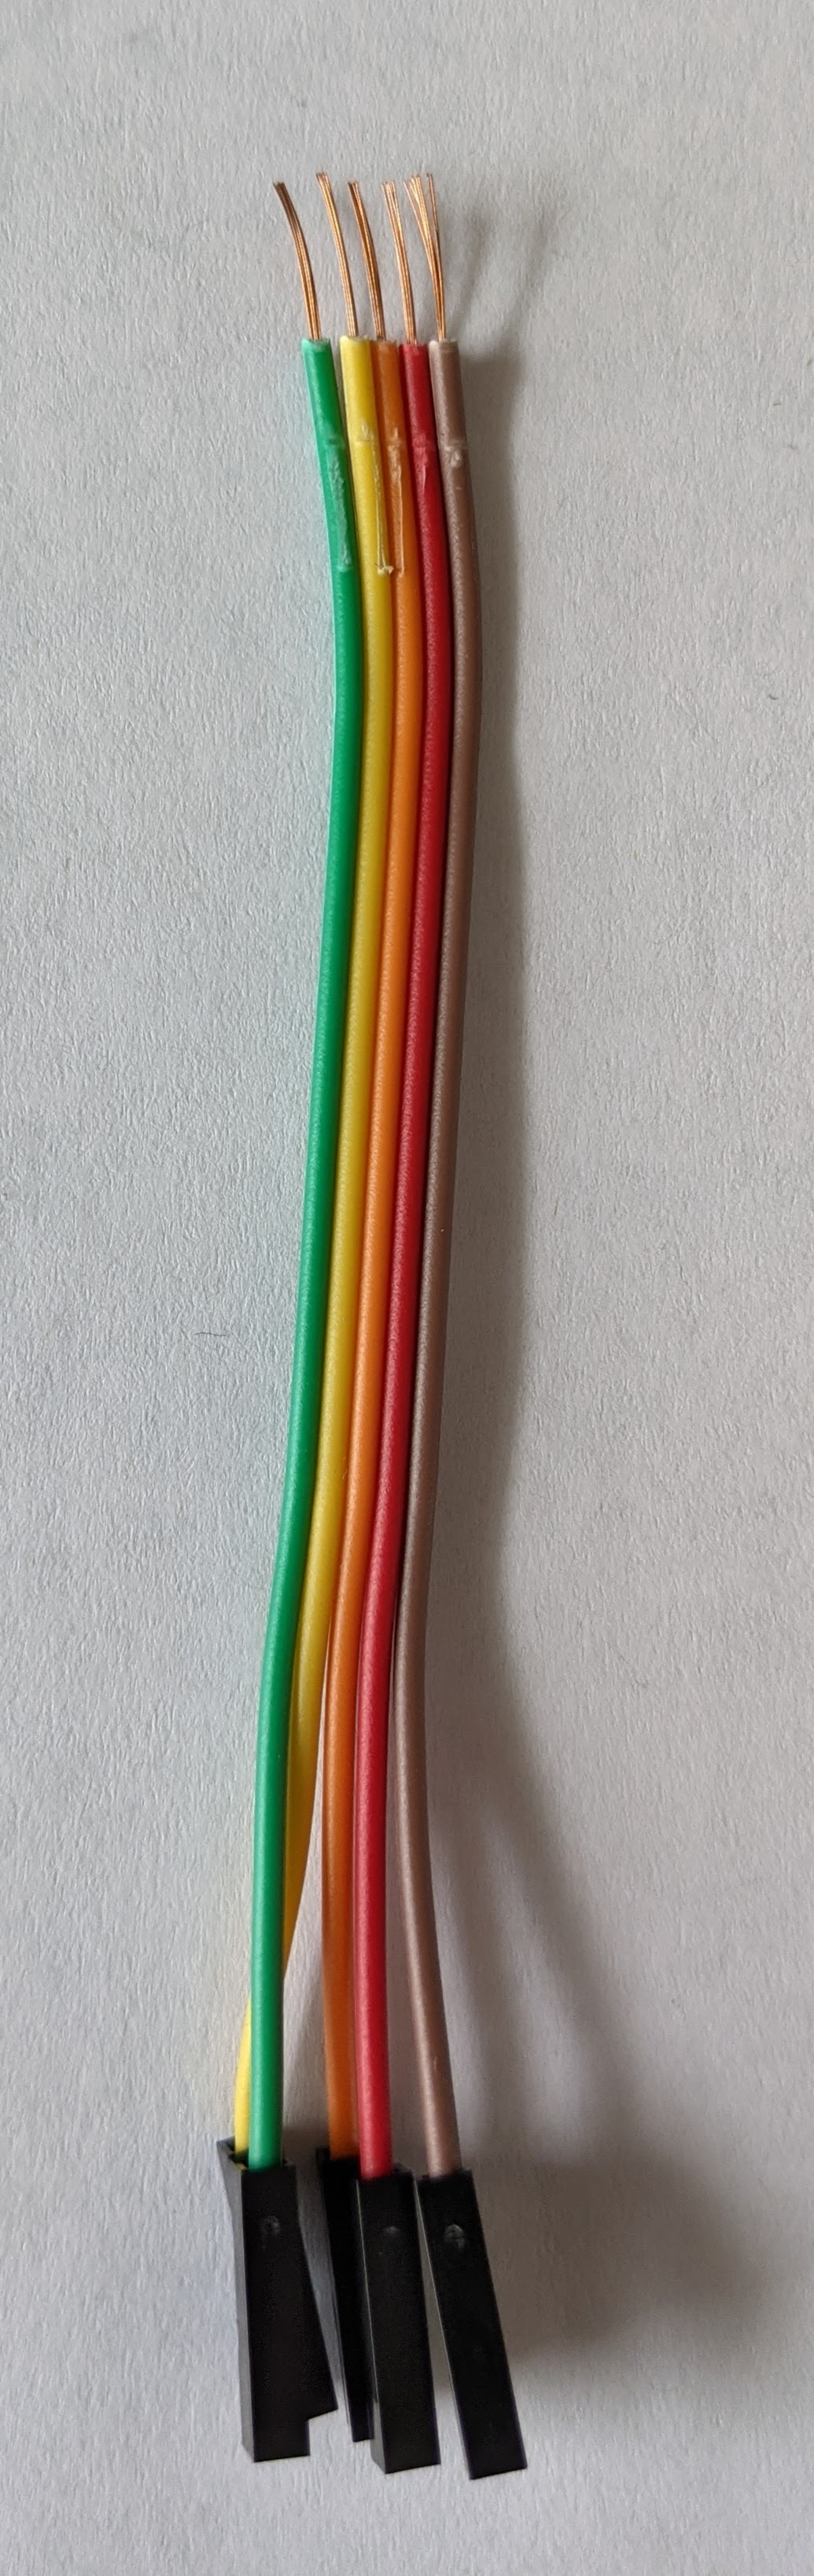
\includegraphics[height=6cm]{./lUltralydtransmitterx0214.jpg}$
$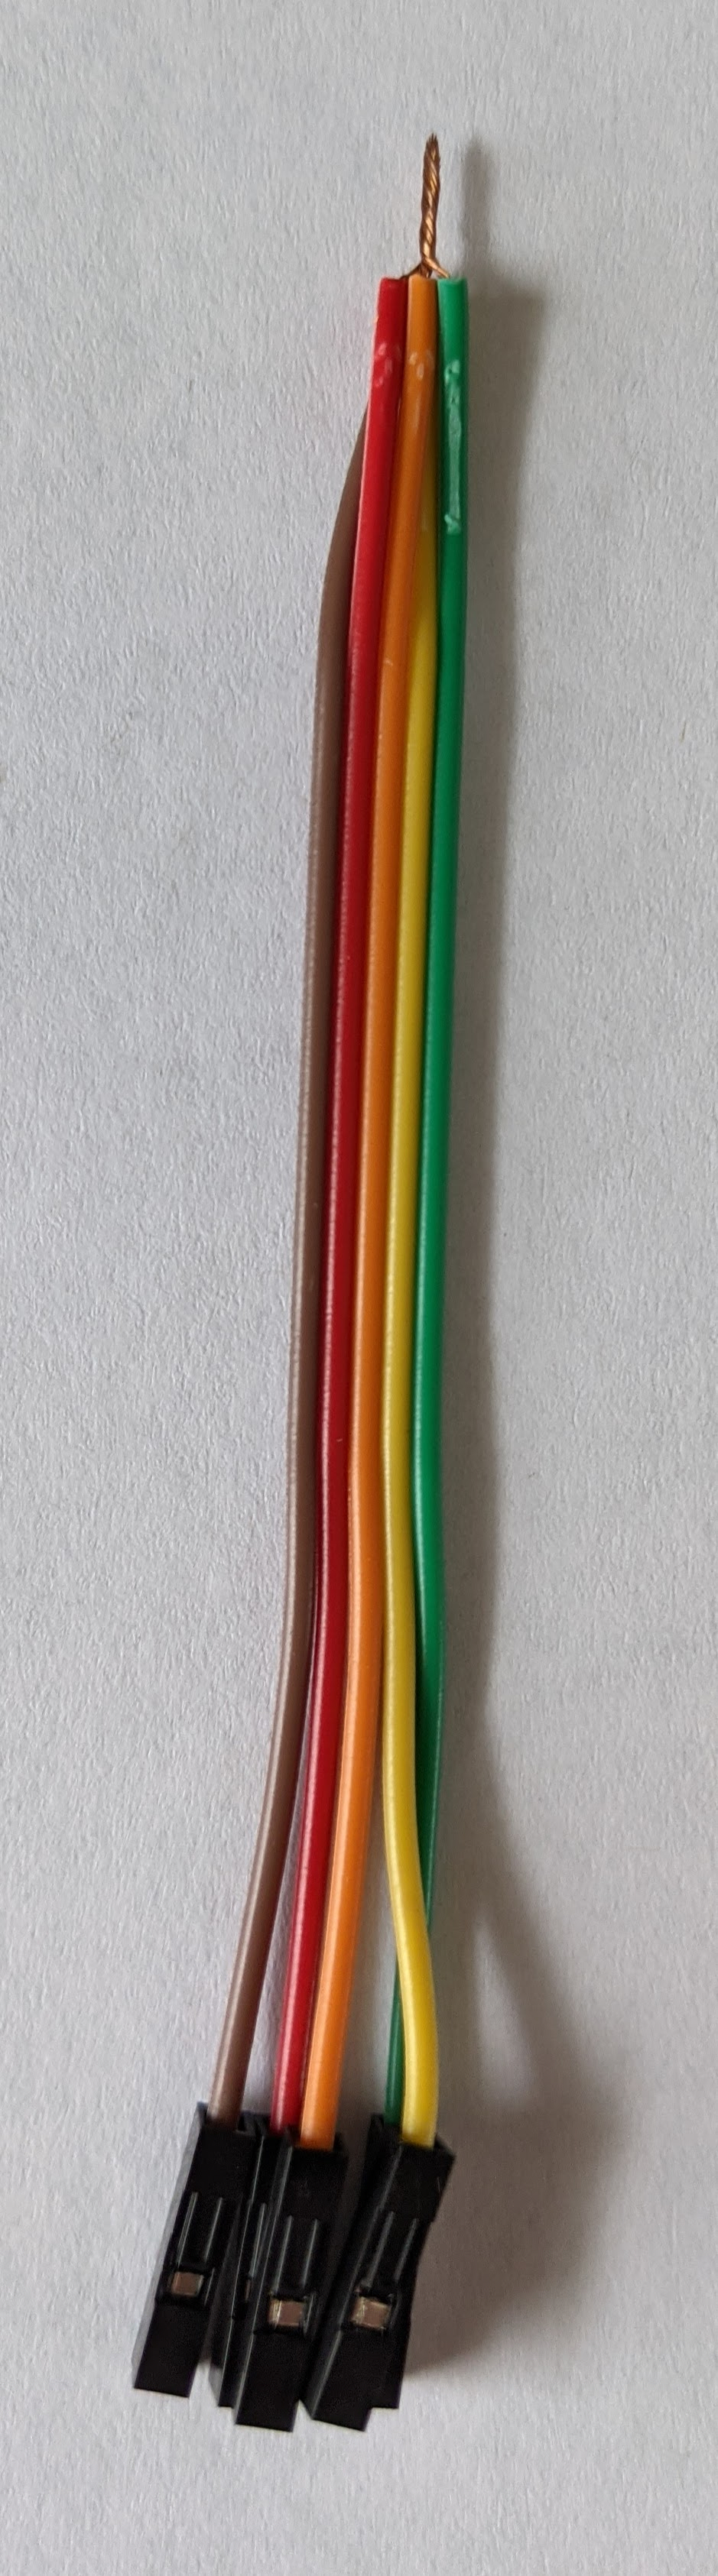
\includegraphics[height=6cm]{./lUltralydtransmitterx0215.jpg}$
$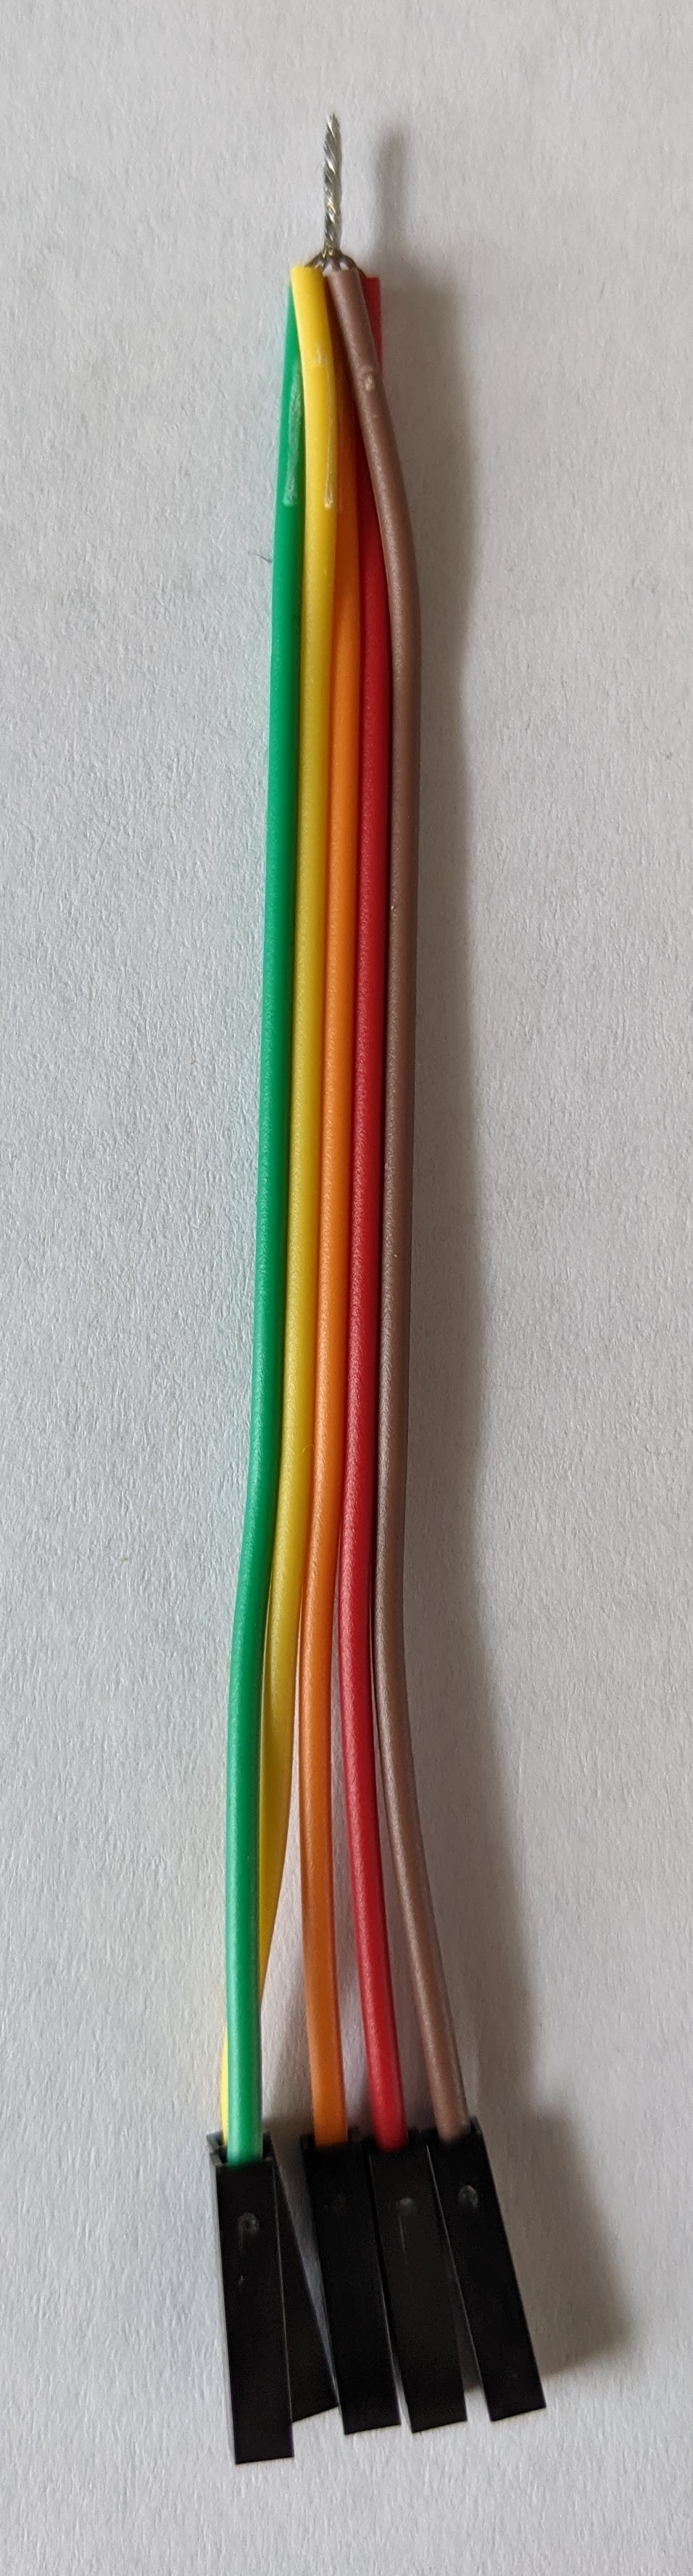
\includegraphics[height=6cm]{./lUltralydtransmitterx0216.jpg}$
$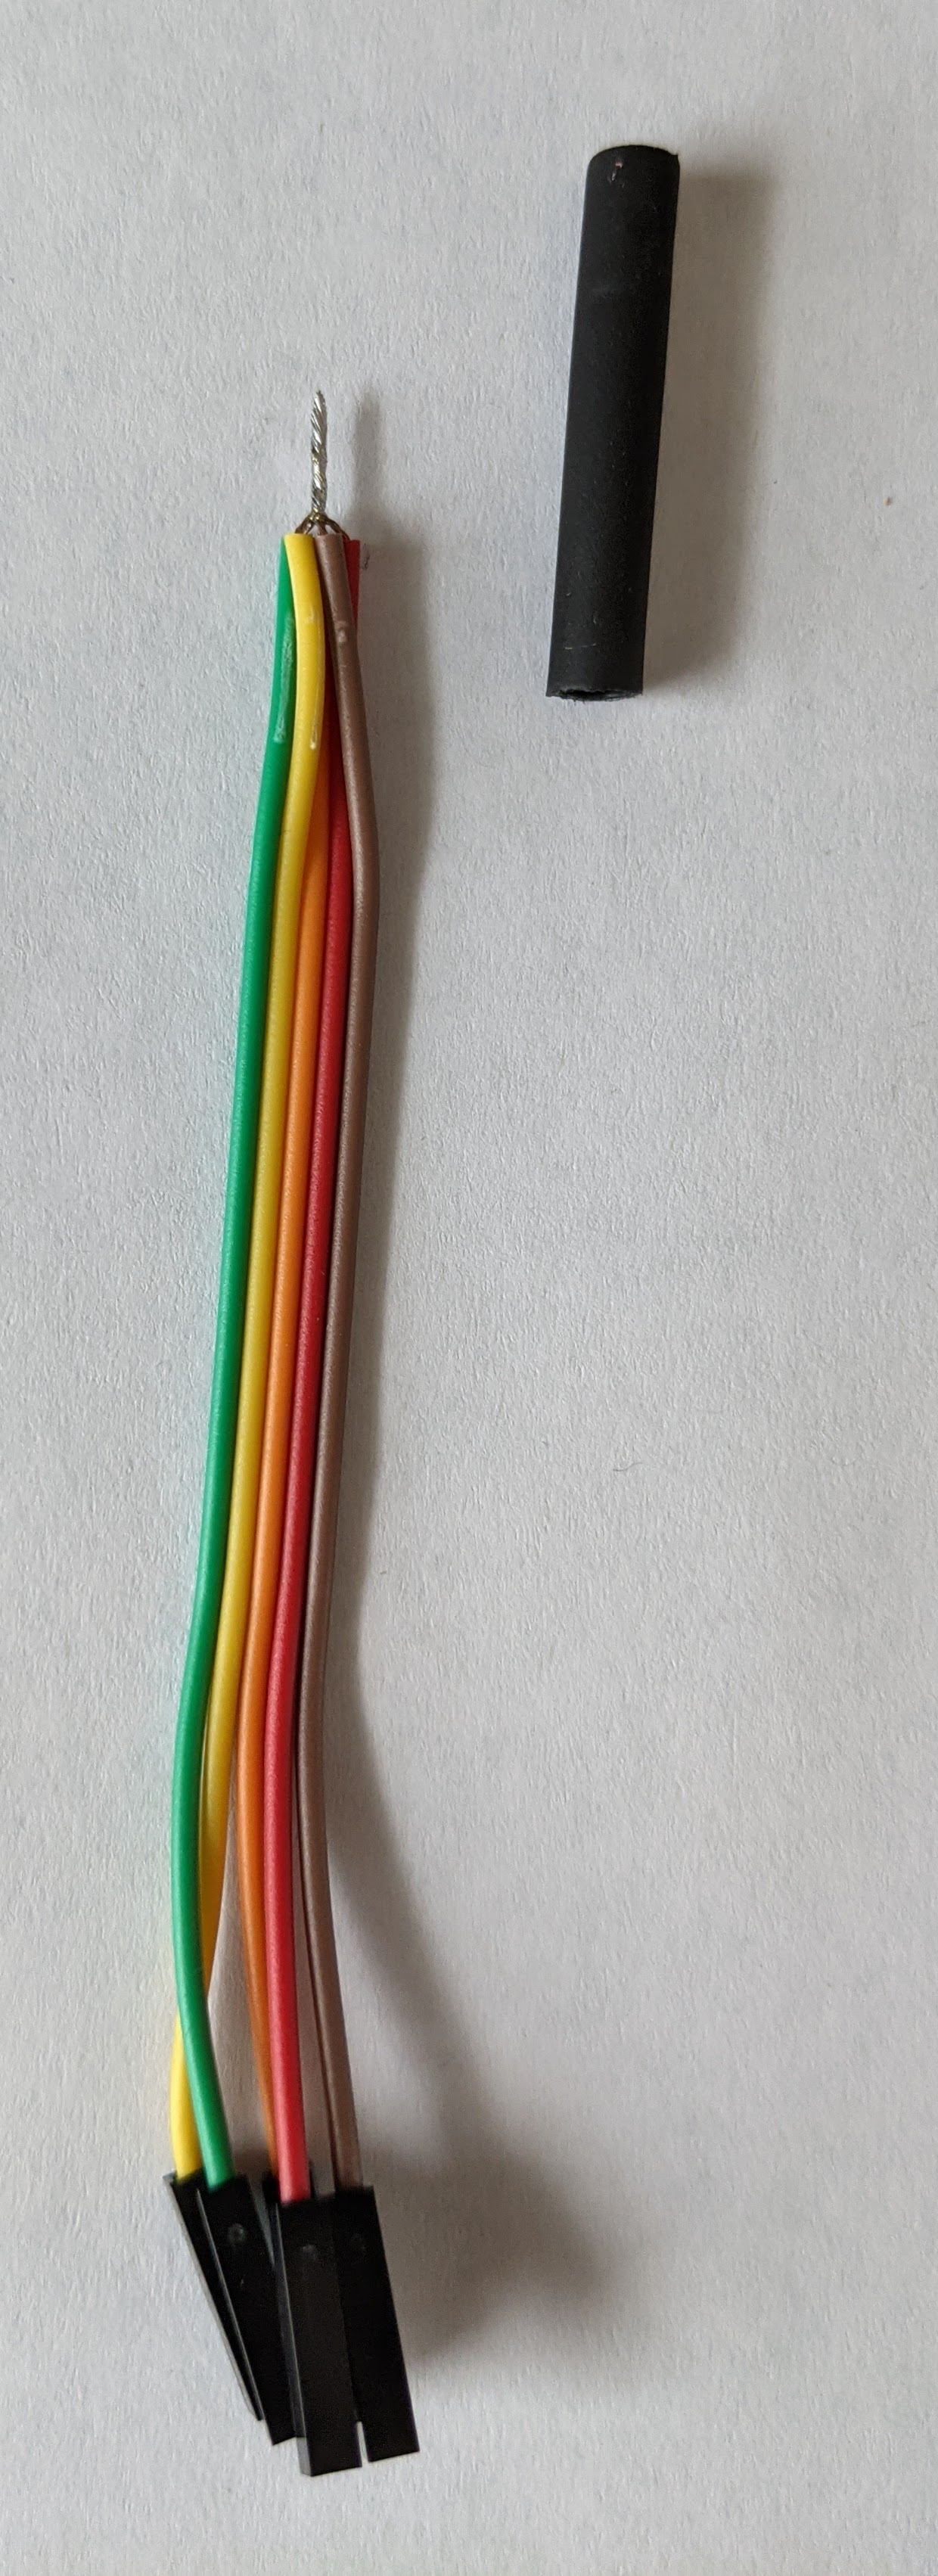
\includegraphics[height=6cm]{./lUltralydtransmitterx0217.jpg}$
$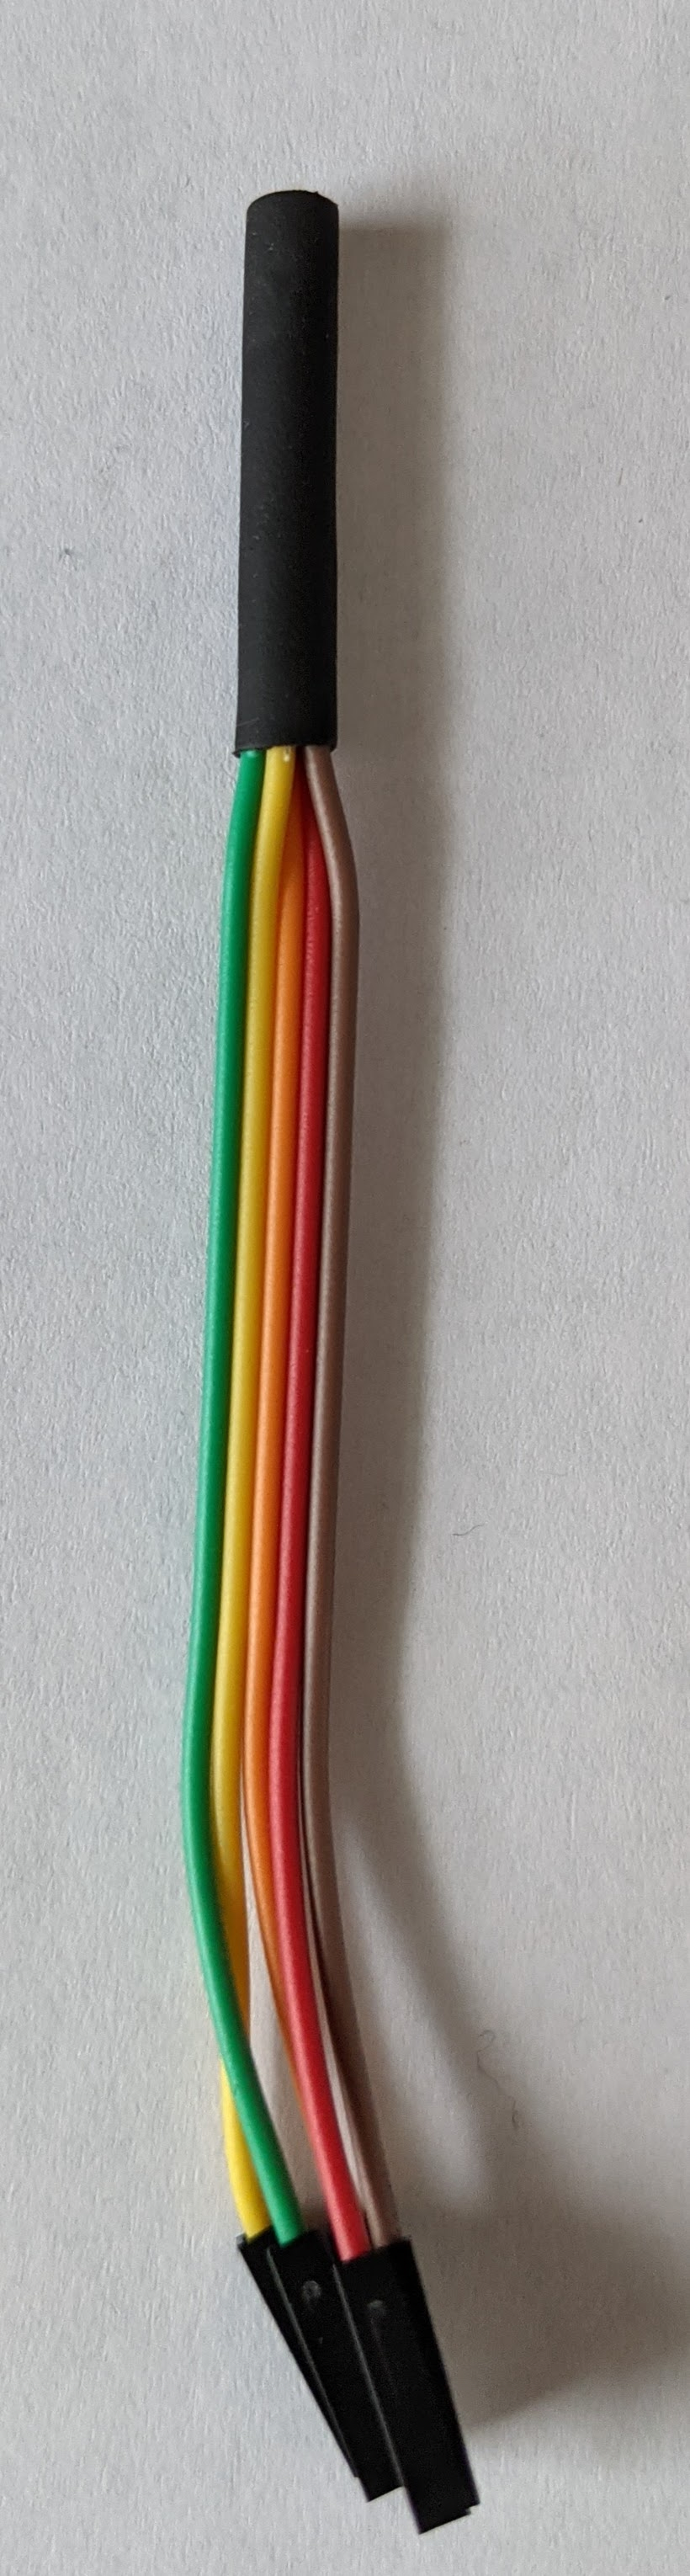
\includegraphics[height=6cm]{./lUltralydtransmitterx0218.jpg}$
$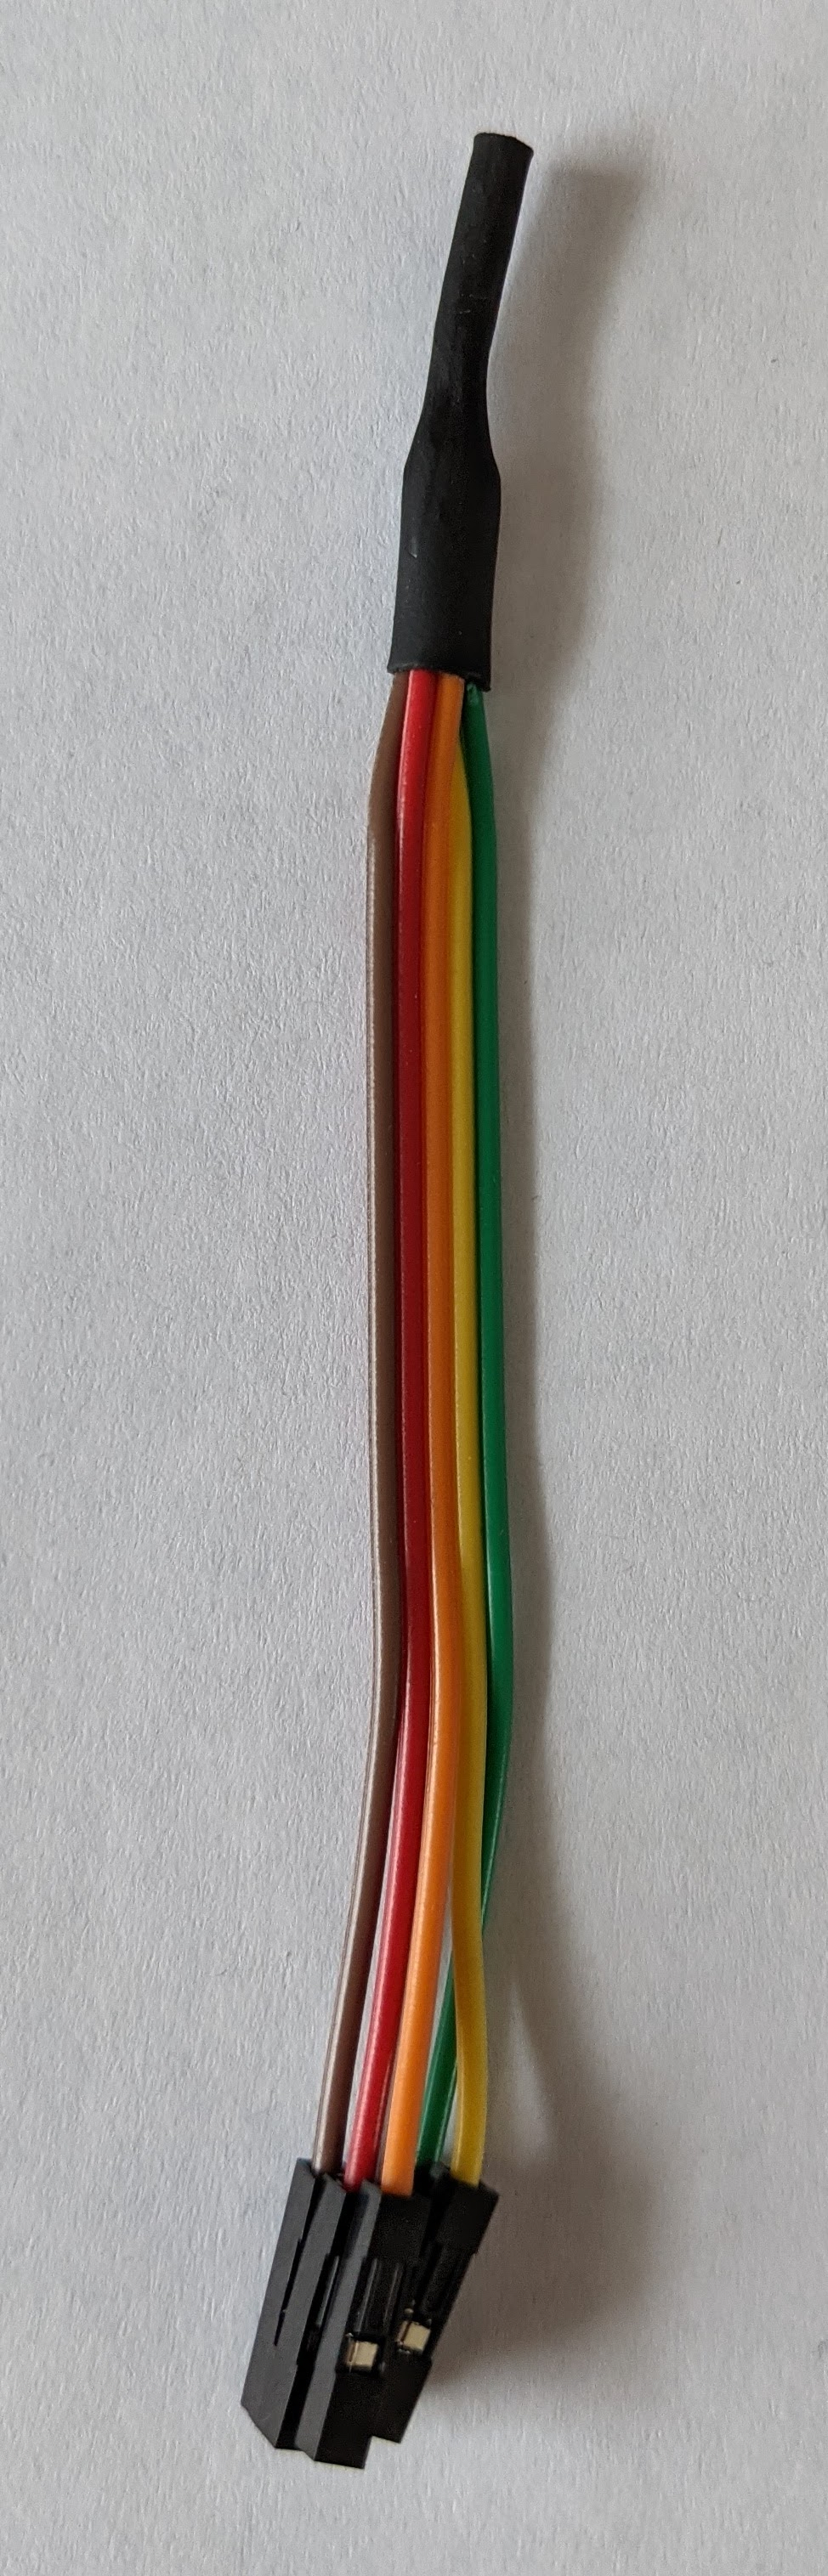
\includegraphics[height=6cm]{./lUltralydtransmitterx0219.jpg}$

\vskip 5pt 

For kunne ta i bruk displayet med arduino må vi ta i bruk tre biblioteker. Legg inn følgende kode før setup delen av programmet. 

\vskip 5pt 
\begin{lstlisting}[language=Arduino]
#include <Wire.h>
#include <Adafruit_GFX.h>
#include <Adafruit_SSD1306.h>

// Declaration for an SSD1306 display connected to I2C (SDA, SCL pins)
#define OLED_RESET     -1 // Reset pin # (or -1 if sharing Arduino reset pin)
Adafruit_SSD1306 display = Adafruit_SSD1306(128, 32, &Wire);
\end{lstlisting}
\vskip 5pt 
Wire biblioteket kommer med arduino IDE, men de to andre må vi installere. Trykk CTRL+SHIFT+I for å åpne bibliotek administrasjon i Arduino IDE. De siste linjene er nødvendige for å deklarere hvordan displayet kobles til og hvor stort det er. 

\vskip 5pt 
Søk først etter GFX og velg Adafruit GFX Library
$$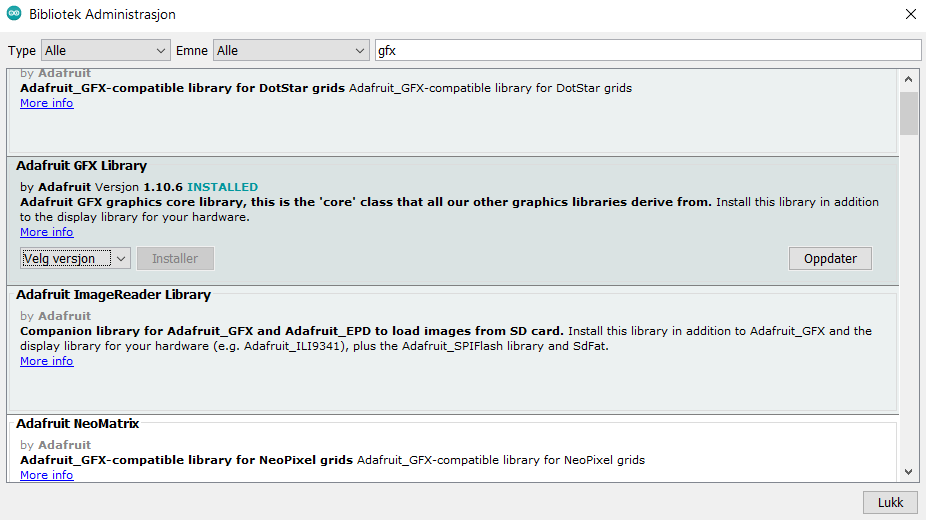
\includegraphics[width=16cm]{./lUltralydtransmitterx0221.png}$$
\vskip 5pt 
Søk deretter etter SSD1306 og velg Adafruit SSD1306
$$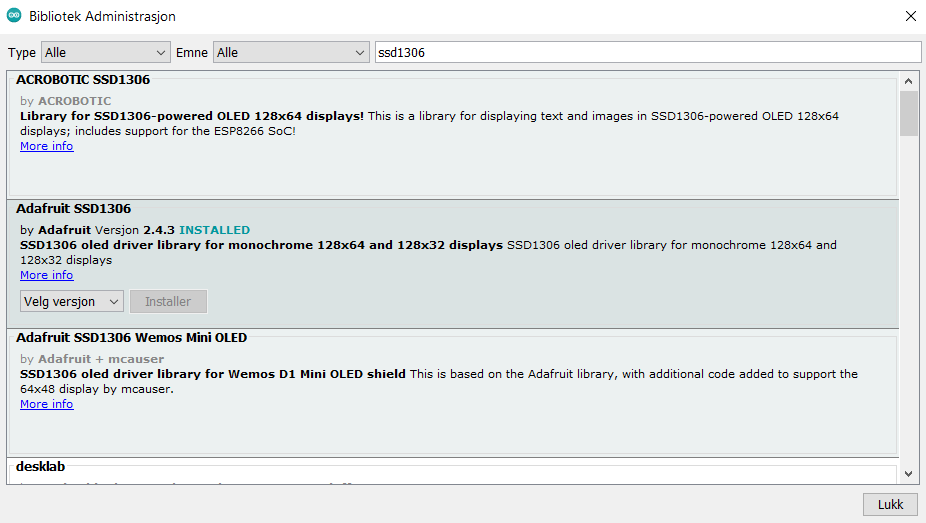
\includegraphics[width=16cm]{./lUltralydtransmitterx0222.png}$$
\vskip 5pt 
I \verb|void setup()| kan du legge til følgende kode. 

\begin{lstlisting}[language=Arduino]
//sette starte displayet og sette inn I2C adressen
display.begin(SSD1306_SWITCHCAPVCC, 0x3C); 
display.clearDisplay();
display.display();
\end{lstlisting}
\newpage
Nå skal du legge inn kode i loop(). Start med koden nedenfor og experimenter selv. 
\begin{lstlisting}[language=Arduino]
// first we clear previous display
display.clearDisplay();
// The size we want
display.setTextSize(1);
// if we du not set som color the display will be black
display.setTextColor(SSD1306_WHITE);
// Where shall we put the new text
display.setCursor(0,0);
//the next 3 lines is displaying the actual text
display.print("Avstand = ");
display.print(distance);
display.print(" cm");
// actually display all of the above
display.display(); 
\end{lstlisting}

\vskip 5pt 
Nå skal du ha et display som viser avstanden til til et objekt forran sensoren. Her kommer noen oppgaver du må finne ut av på egen hånd.
\begin{enumerate}
	\item Legg koden som skal til for å måle og skrive til displayet inn in en funkson slik at du i loop koden bare trenger å kalle:
	\begin{lstlisting}[language=Arduino]
	meassure();
	\end{lstlisting}
	\item konverter koden til å kunne måle nivået i en tank. For å teste kan du f.eks. sette sensoren mot gulvet fra  pulten og la dette være null nivå. Så skal nivået øke jo lengre et objekt kommer mot sensoren. Du kan gjerne teste ved å holde en bok imellom. 
	\item Utvid programmet slik at det bare måler nivået og skriver dette til skjermen hvert 100ms. 
\end{enumerate}



\underbar{file ./lUltralydtransmitter.tex}
\end{document}

